\chapter{Le réseau local}
Un \textit{réseau local}, ou LAN (\textit{Local Area Network}) est de taille modeste. Les équipements qui y sont connectés s'envoient des données entre eux sans passer par internet. Un bon exemple de LAN est le \textit{réseau domestique} d'une maison :
\begin{itemize}
    \item    la box, fournie par l'opérateur (Orange, Free, Bouygues...) fait office de switch et de routeur;
    \item    les téléphones portables, tablettes, ordinateurs, imprimantes et autres s'y intègrent.
\end{itemize}
\begin{center}
    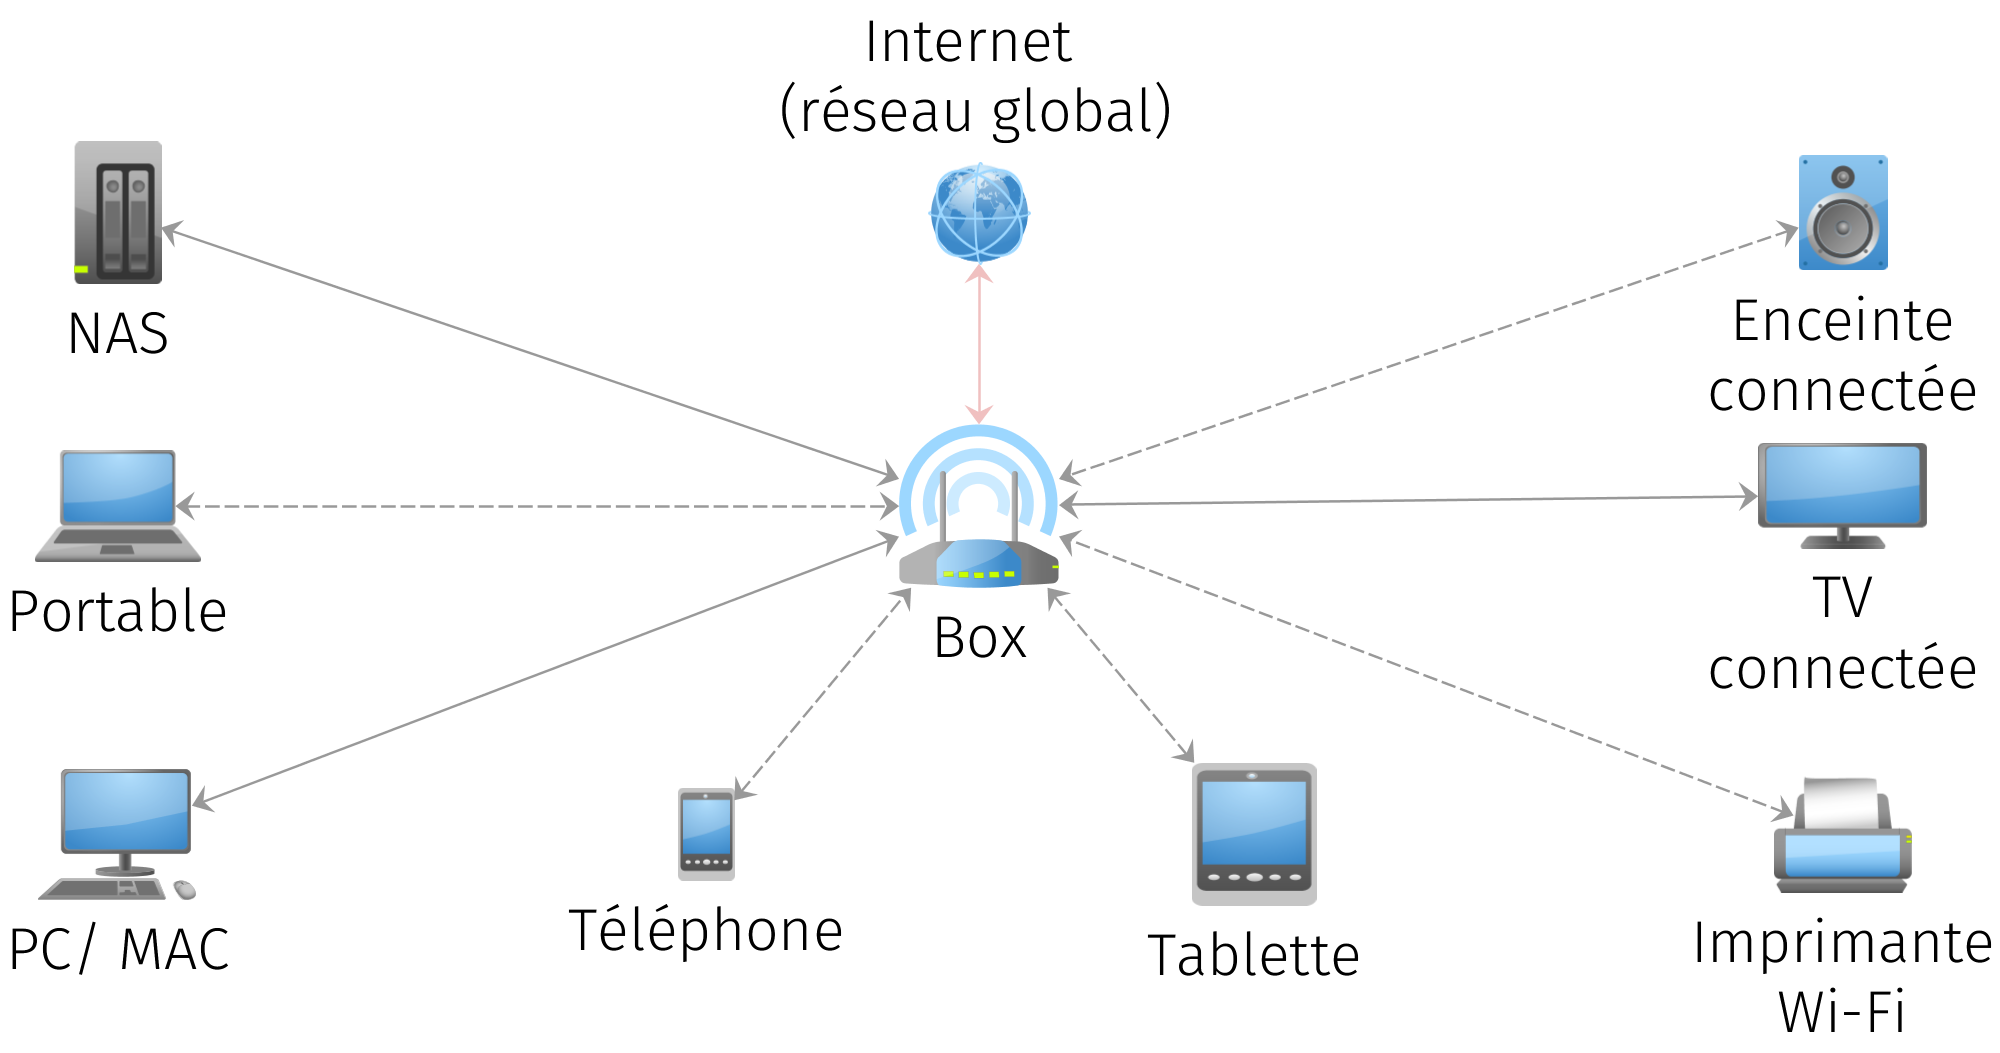
\includegraphics[width=\textwidth]{ch-reseaulocal/img/reseau_local.png}
\end{center}

\section{Les adresses IP privées et publiques}
On a vu dans le chapitre précédent l'importance de l'adresse IP d'un ordinateur dans le rôle de la communication.

\begin{definition}[ : adresse IPv4]
    Une adresse IP (version 4) est la donnée de 4 octets. On les note séparés par des points. Il y a 5 classes d'adresse IP, notées A, B, C, D et E et les 3 premières classes disposent d'adresses IP (on abrègera en IP) publiques et privées.
\end{definition}

\begin{exemple}[s]
    \begin{itemize}
        \item    74.125.21.138 est à ce jour une IP permettant d'accéder au site du moteur de recherche de Google. C'est une IP \textit{publique}, accessible par tout le monde \textit{via} Internet.\\
        \item    192.168.1.47 est l'IP de l'ordinateur sur lequel j'écris ces lignes. C'est une IP \textit{privée} : elle n'est accessible que par les ordinateurs de mon propre réseau domestique. Elle n'est d'ailleurs pas \textit{unique} non plus dans le sens où d'autre réseaux domestiques utilisent cette IP.
        \item    lorsque je veux voir mon IP publique, je vais par exemple consulter \texttt{http://whatismyip.host/} et je trouve une adresse différente : 83.199.117.xx (permettez moi de garder mon adresse IP secrète).
    \end{itemize}
\end{exemple}

Une adresse IP publique, c'est un peu comme une adresse postale publique : elle identifie de manière unique une machine (qui peut être une box jouant le rôle de routeur vers un réseau domestique).\\
Une adresse IP privée, c'est un peu comme le numéro et le nom de la rue sans la ville ni le pays : il y a sans doute beaucoup d'adresse au 24 rue des oliviers. Si le réseau postal ne concerne que la ville de Rennes, cette adresse est suffisante, mais si je cherche à envoyer du courrier au 24 rue des oliviers, cela ne marchera pas.

\begin{remarque}[s]
    \begin{itemize}
        \item    4 octets pour une adresse IP, c'était bien il y a 30 ans, ça l'est beaucoup moins de nos jours !\\ $2^{32}=\np{4 294 967 296}$, donc vu le nombre de machines croissant en fonctionnement simultané sur Terre, il est impossible d'attribuer une IP unique à chaque ordinateur connecté à Internet, d'où l'importance du LAN.

        \item    Pour pallier le problème, une norme IP version 6, plus performante, sur 128 bits au lieu de 32, a vu le jour mais peine encore à s'imposer.
    \end{itemize}
\end{remarque}

Voici les plages d'IP publiques et privées selon les classes :
\begin{itemize}[]
    \item    \textbf{Classe A :} de l'adresse IP 0.0.0.0 à 126.255.255.255.\\
          Adresses privées : de 10.0.0.0 à 10.255.255.255 (avec 16 millions d'adresses possibles au sein d'un réseau local).

    \item    \textbf{Classe B :} de l'adresse IP 128.0.0.0 à 191.255.255.255.\\
          Adresses privées : 172.16.0.0 à 172.31.255.255 (avec 65535 adresses possibles au sein d'un réseau local).
    \item    \textbf{Classe C :} de l'adresse IP 192.0.0.0 à 223.255.255.255.\\
          Adresses privées C : 192.168.1.0 à 192.168.255.255 (255 adresses possibles dans un réseau local).
    \item    \textbf{Classe D (réservée) :} de l'adresse IP 224.0.0.0 à 239.255.255.255.
    \item    \textbf{Classe E (réservée) :} de l'adresse IP 240.0.0.0 à 255.255.255.255.
\end{itemize}

\begin{exemple}[]
    Mon adresse IP publique est une IP de classe A, mon IP privée est de taille C, ce que je comprends parfaitement puisque mon réseau domestique ne contiendra qu'une dizaine de terminaux tout au plus.
\end{exemple}


\section{L'exemple du réseau local traditionnel}

Lorsqu'on met en place un réseau local, on commence par déterminer sa taille. Il y a beaucoup de chances qu'on ait moins de 256 machines à connecter donc on va choisir une IP publique de classe C :
\begin{itemize}
    \item    je choisis de prendre pour \textit{adresse réseau} 192.168.1.0, ce n'est pas une IP attribuée à une machine, elle désigne mon réseau local ;
    \item    le \textit{masque de sous-réseau} par défaut est 255.255.255.0, ce qui signifie que les 3 premiers octets des machines de mon réseau sont « bloqués » et donc que les machines vont avoir des adresses du type 192.168.1.xx ;
    \item    je peux attribuer des IP aux machines que je veux connecter, par exemple 192.168.1.1 pour la première, et c\ae tera ;
    \item    la dernière IP 192.168.1.255 est interdite, elle est réservée pour adresser un message à l'ensemble des machines du réseau (on appelle ceci \textit{broadcast}).
\end{itemize}

\begin{remarque}[]
    Prenons le cas d'un foyer qui utilise le FAI Orange. Par défaut le réseau local est 192.168.1.0. avec pour masque 255.255.255.0. La LiveBox, qui fait office de switch et de routeur, a pour adresse 192.168.1.1. C'est cette adresse qui est utilisée comme passerelle pour accéder à internet :
    \begin{center}
        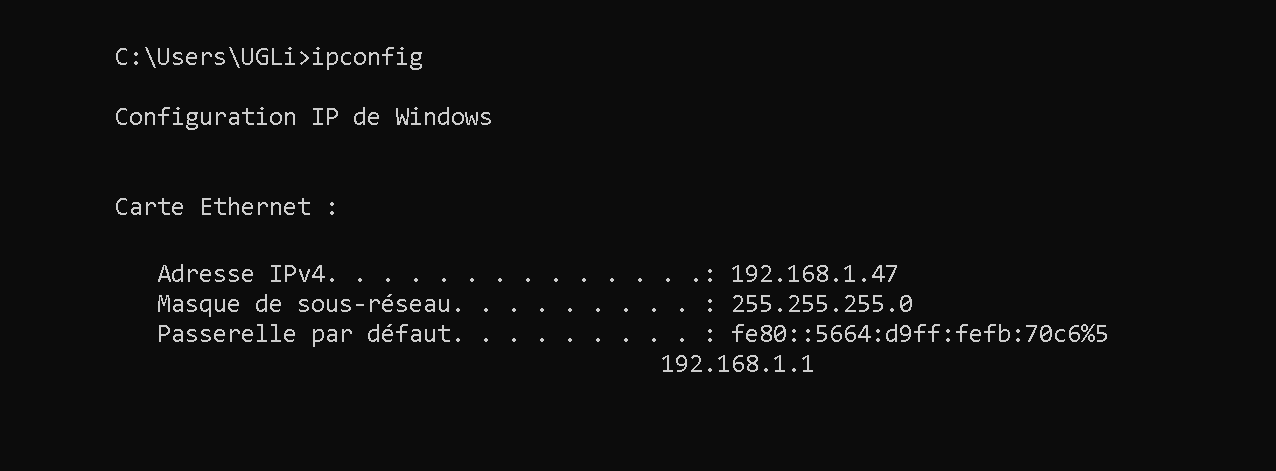
\includegraphics[width=\textwidth]{ch-reseaulocal/img/ipconfig.png}
    \end{center}

    La commande\texttt{ipconfig} de Windows (\texttt{ifconfig} sous Linux et Mac) me permet de retrouver ces informations ainsi que mon IP privée.
\end{remarque}
\begin{exercice}[]
    Utilise l'invite de commande de ton système d'exploitation (touche windows et taper\texttt{cmd} pour Windows, Terminal sous MacOS) et trouve l'IP de ton ordinateur, le masque de sous-réseau et l'adresse de la passerelle.
\end{exercice}
\section{Un outil de simulation réseau : Filius}

Filius est un logiciel libre fonctionnant sur tous les systèmes d'exploitation et permettant de simuler le fonctionnement d'un petit réseau. On peut
\begin{itemize}
    \item    ajouter du matériel : ordinateur, switch, routeur et modem;
    \item    connecter les éléments précédents;
    \item    configurer ces éléments;
    \item    installer de petites applications sur les ordinateurs connectés pour transmettre ou recevoir des données sur le(s) réseau(x).
    \item    visualiser les échanges de données.
\end{itemize}

Nous utiliserons Filius pour observer ce que nous avons appris des réseaux.


